\documentclass[5pt]{article}
\usepackage{mathptmx,amsmath}
\usepackage{pdfslide2,pause}
\usepackage{eurosym}
\usepackage[portuguese,english]{babel}
\usepackage{kerkis}
\usepackage{colortbl} % used to highlight row or columns of tables. http://www.tug.org/pracjourn/2007-1/mori/mori.pdf
\usepackage[small]{caption} % more option on http://www.dd.chalmers.se/latex/Docs/PDF/caption.pdf
\usepackage[tight,scriptsize]{subfigure}
\usepackage{lastpage}
\usepackage{chngcntr}
\usepackage[absolute,overlay]{textpos}
\usepackage{tabto}
\usepackage{animate}
\usepackage{listings}
\captionsetup{labelformat=empty,skip=-0.8cm}


%\lstset{
%    language=Matlab,                % choose the language of the code
%    basicstyle=\ttfamily\tiny,       % the size of the fonts that are used for the code
%    numbers=none,                   % where to put the line-numbers
%    numberstyle=\tiny,              % the size of the fonts that are used for the line-numbers
%    stepnumber=1,                   % the step between two line-numbers. If it's 1 each line will be numbered
%    numbersep=5pt,                  % how far the line-numbers are from the code
%    backgroundcolor=\color{white},  % choose the background color. You must add \usepackage{color}
%    showspaces=false,               % show spaces adding particular underscores
%    showstringspaces=false,         % underline spaces within strings
%    showtabs=false,                 % show tabs within strings adding particular underscores
%    tab=\rightarrowfill,
%    frame=none,	                    % adds a frame around the code
%    tabsize=2,	                    % sets default tabsize to 2 spaces
%    captionpos=b,                   % sets the caption-position to bottom
%    breaklines=true,                % sets automatic line breaking
%    breakatwhitespace=false,        % sets if automatic breaks should only happen at whitespace
%    title=\lstname,                 % show the filename of files included with \lstinputlisting; also try caption instead of title
%    escapeinside={\%*}{*)},          % if you want to add a comment within your code
%    morekeywords={ifftshift,fftshift},
%    keywordstyle=\bfseries\color[rgb]{0,0,0.3},
%    commentstyle=\color[rgb]{0.133,0.5,0.133}
%}
%\lstset{
%    emph={function,end,for,if,while},
%    emphstyle=\bfseries\color[rgb]{0.6,0,0},
%}

\definecolor{itblue}{rgb}{0.0,0.0,0.5}
\definecolor{itred}{rgb}{0.82,0.18,0.24}
\newcommand{\pageNum}{
    \begin{picture}(0,0)(0,0)
        \put(-15,-390){
            \begin{minipage}{1.8cm}
            \end{minipage}
        }
    \end{picture}
}
\newcommand{\cb}[1]{{\color{itblue} #1}}%
\newcommand{\cred}[1]{{\color{itred} #1}}%
\newcommand{\bb}[1]{{\textbf{\color{itblue} #1}}}%
\newcommand{\br}[1]{{\textbf{\color{itred} #1}}}%
\renewcommand{\labelitemi}{\textcolor{itred}{\normalsize $\bullet$}}
\renewcommand{\labelitemii}{\textcolor{itblue}{$\bullet$}}
\newcommand{\mysection}[1]{\section*{\pageNum\color{itred}\sffamily #1}\vspace*{0.5cm}\overlay{it_1.png}\sffamily}%
\newcommand{\ITfootnote}[1]{\hspace{1.8cm}\begin{minipage}{13cm}\tiny{#1}\end{minipage}}
\newcommand{\edfaGain}{$G=\exp\left(\frac{\alpha}{2}L_{span}\right)$}
\newenvironment{reference}{
    \begin{textblock*}{0.7\textwidth}(32mm,137mm)\tiny\noindent\bgroup\color{black}
}
{
    \egroup\end{textblock*}
}


\graphicspath{{./Figures/}}
\pagestyle{title}

\hyphenpenalty=50000
\tolerance=10000

\setlength{\textheight}{1.5\textheight}

%%%%%%%%%%%%%%%%%%%%%%%%%%%%%%%%%%%%%%%%%%%%%%%%%%%%%%%%%%%%%%%%%%%%%%%%%%%%%%%%%%%%%%%%%%%%%%%%%%%
%%%%%%%%%%%%%%%%%%%%%%%%%%%%%%%%%%%%%%%%%%%%%%%%%%%%%%%%%%%%%%%%%%%%%%%%%%%%%%%%%%%%%%%%%%%%%%%%%%%

\begin{document}

%************************************************************************************************
%                                          SLIDE
%************************************************************************************************
\pagenumbering{roman}
\begin{titlepage}  \overlay{it_0.png}

\color{itblue} \sffamily \noindent \small
\hspace*{1cm}  Quantum Technologies\\
\hspace*{1cm}  Physics Department, University of Aveiro,\\ %Instituto\\ Superior T�cnico, Instituto de Telecomunica��es\\
%
\hspace*{1cm}  2018-2019\\ 

\vspace*{1cm}
\begin{center}
    \color{black} \sffamily \noindent \Large
    \br{Coherent One Way (COW) QKD Protocol \\}
\end{center}
\vspace{6mm}
\begin{center}
    \color{black}
    \textbf{João António$^1$, Daniel Pereira$^{2,3}$, Armando N. Pinto$^{2,3}$\\}
    {}
\end{center}

\vspace{0.0mm}
\scriptsize
\begin{center}
Physics Department$^1$,\\
Department of Electronics, Telecommunications and Informatics$^2$,\\
University of Aveiro, Aveiro, Portugal\\
Instituto de Telecomunica\c{c}\~{o}es,$^3$, Aveiro, Portugal\\
\end{center}

\vspace{1.0cm}
\hspace*{13.2cm}\tiny \copyright 2005, it - instituto de telecomunica\c{c}\~{o}es\hfill

\end{titlepage}


\renewcommand{\headsep}{-25pt}
\pagenumbering{arabic}

%--------------------------------------------------------------------------------------------------
%------------ SLIDE -------------------------------------------------------------------------------

\mysection{Quantum Key Distribution}\large
\vspace*{0.5cm}
Quantum Key Distribution (QKD) is a secure way of sharing a unique random key (composed of 0 and 1) between two parties spatially distant. They later use this symmetric key to encrypt and decrypt messages between them.

To share/create the random key, they use two channels, one quantum channel and one Authenticated classic channel (can be eavesdropped but can't be modified).

  \begin{figure}[hbt]
    	\centering
    	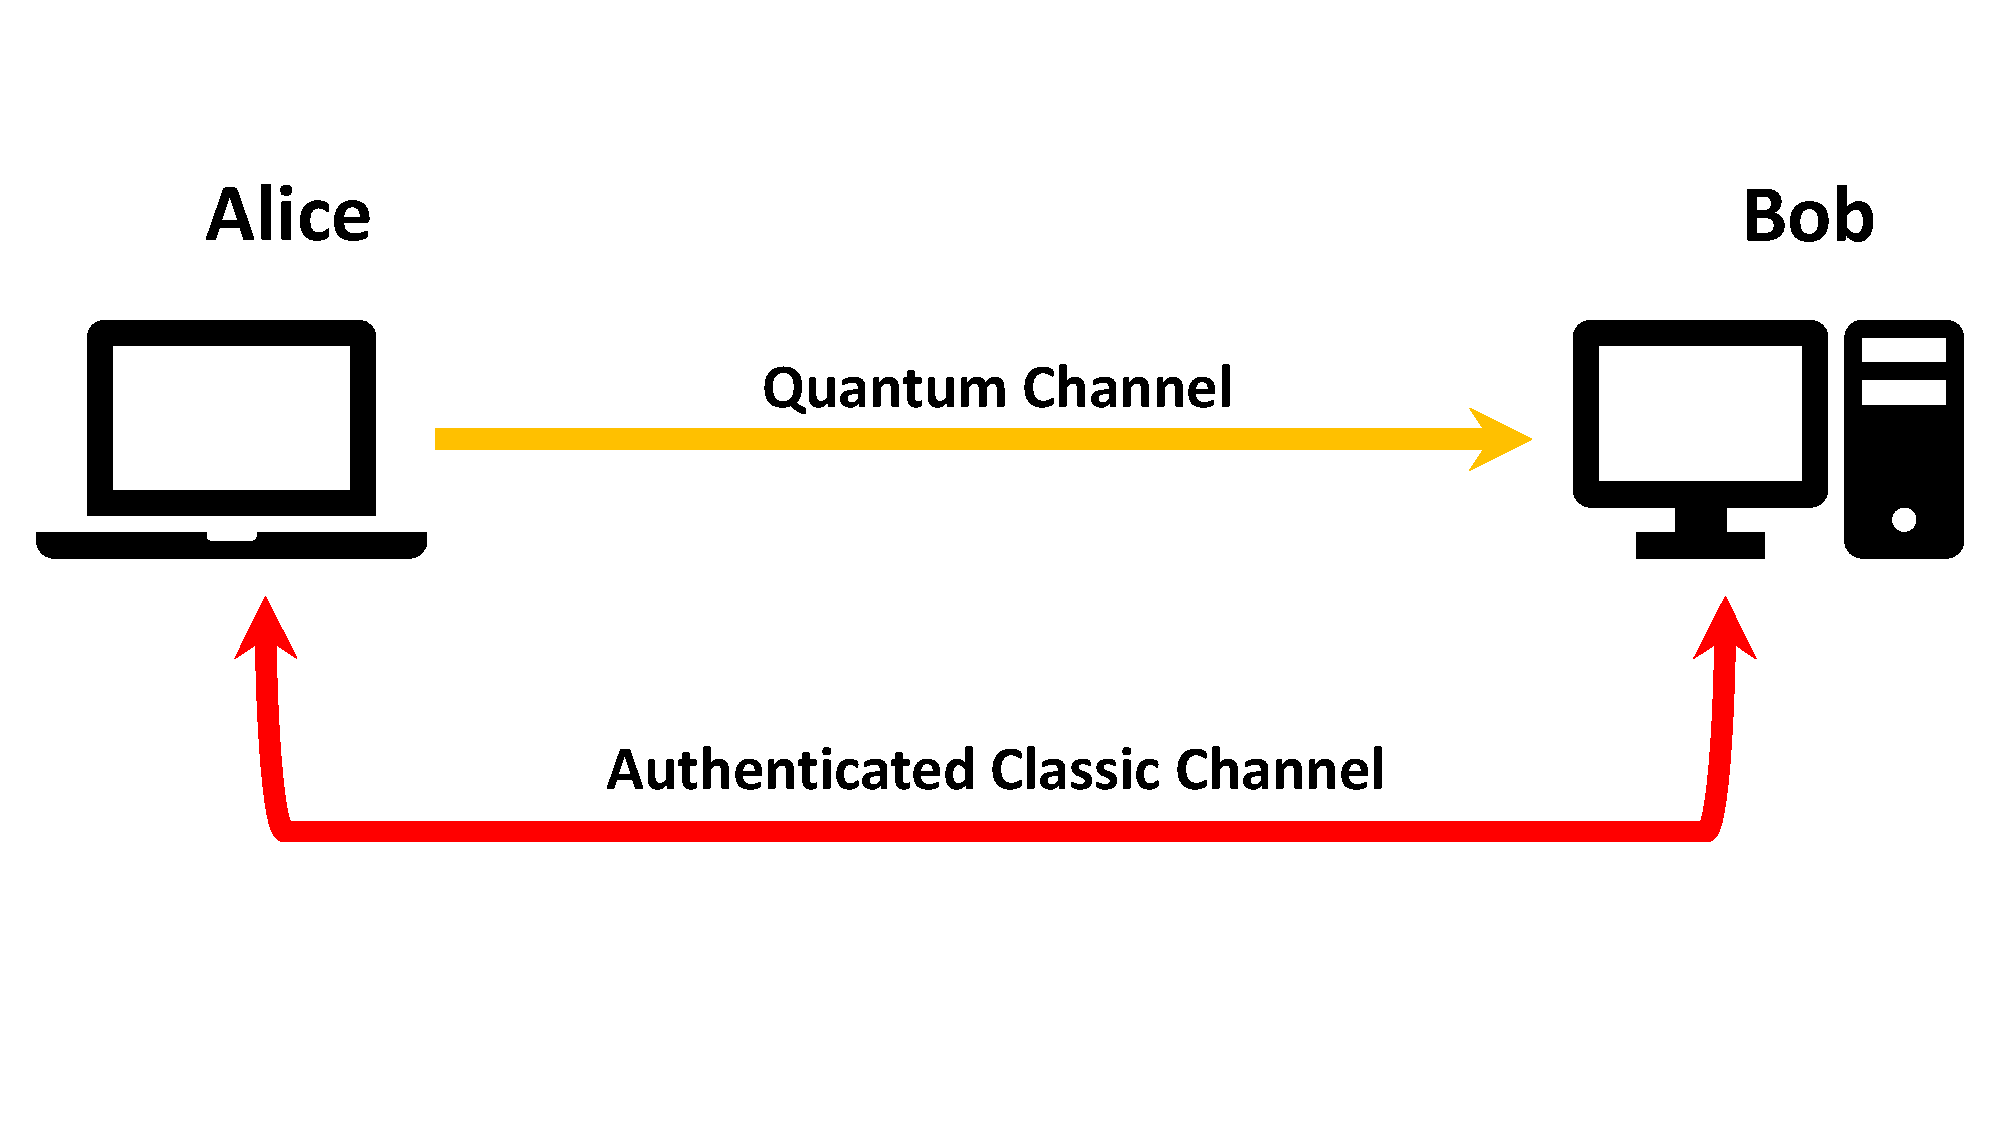
\includegraphics[width=0.6\textwidth]{./figures/All.pdf}
        	\label{All}
    \end{figure}

%--------------------------------------------------------------------------------------------------
%------------ SLIDE -------------------------------------------------------------------------------

\mysection{Quantum Key Distribution}\large
\vspace*{1cm}
The two main types of QKD are Polarization protocols and Time Bin protocols.

The Coherent One Way (COW) protocol was elaborated by Nicolas Gisin et al in 2004 [1]. 
Uses time bin properties.

It is also characterized by having a very simple experimental setup since Bob's apparatus is passive.

    \begin{figure}[hbt]
    	\centering
    	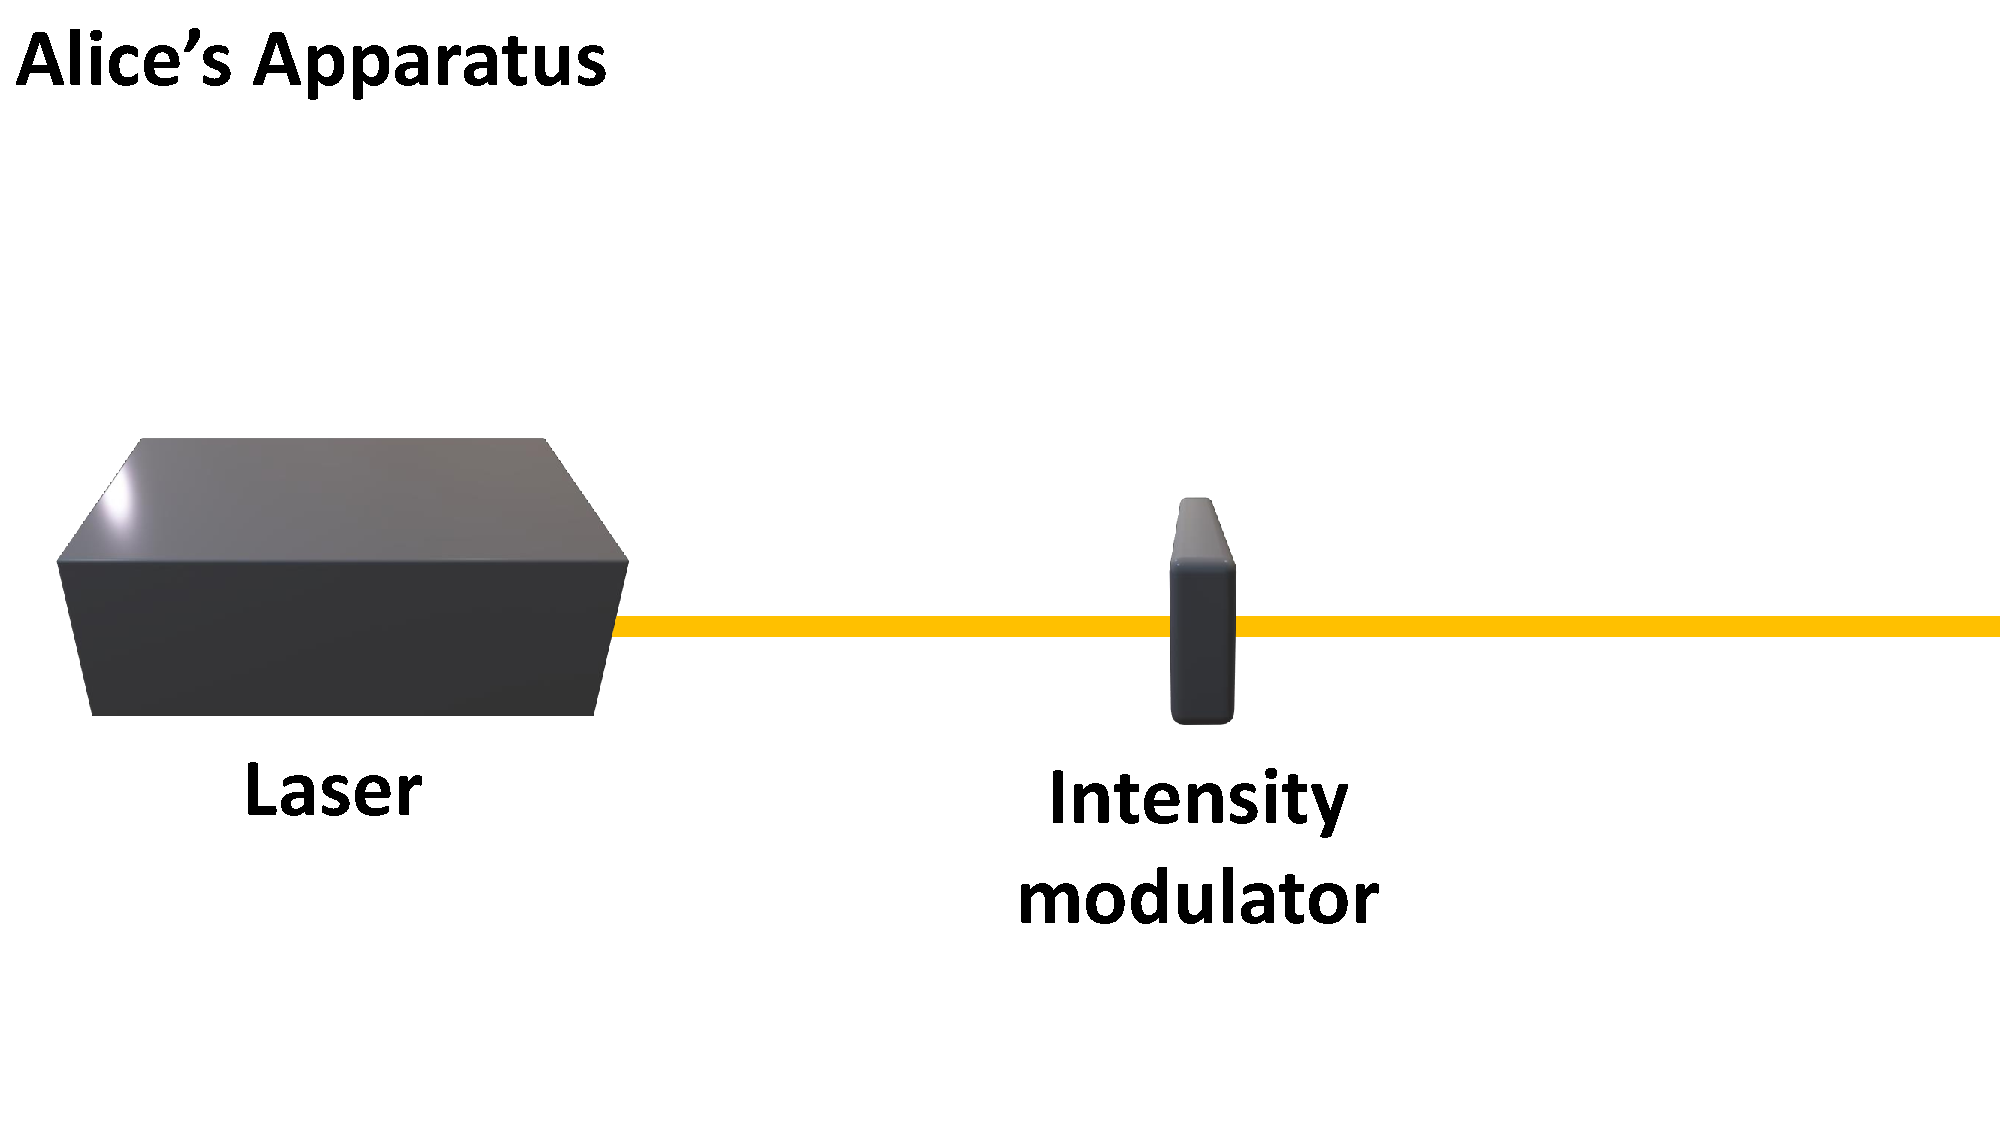
\includegraphics[width=0.6\textwidth, height=5cm]{./figures/Alice.pdf}
        	\label{bob}
    \end{figure}

[1] Gisin, Nicolas, et al. "Towards practical and fast quantum cryptography." arXiv preprint quant-ph/0411022 (2004).

%--------------------------------------------------------------------------------------------------
%------------ SLIDE -------------------------------------------------------------------------------

\mysection{COW - Protocol}\large
\vspace*{0.3cm}

\begin{description}
  \item[Step 1] Alice creates a random key using:  
    \small
$$|0\rangle = |\alpha\rangle |\emptyset\rangle$$      
  $$|1\rangle = |\emptyset\rangle |\alpha\rangle$$
$$|d\rangle = |\alpha\rangle |\alpha\rangle$$
\normalsize
Where $|\emptyset\rangle$ is the vacuum state and $|\alpha\rangle$ is a coherent state of light with intensity $\mu=|\alpha|^2$ and spreads a few random decoy states ($|d\rangle$) in random locations during the creation of the key.
      
  \begin{figure}[hbt]
    	\centering
    	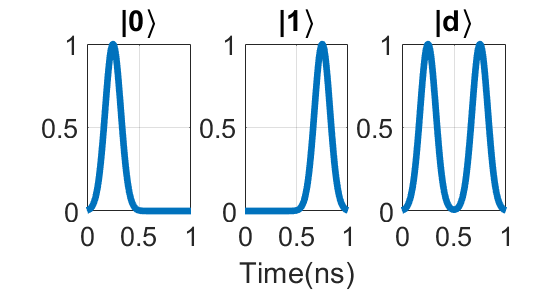
\includegraphics{./figures/Simple.png}
        	\label{Simple}
    \end{figure}

\end{description}

%--------------------------------------------------------------------------------------------------
%------------ SLIDE -------------------------------------------------------------------------------

\mysection{COW - Protocol}\large

\begin{description}
  \item[Step 2] Bob's detection is completely passive. An asymmetric coupler sends a fraction $t_B$ of the photons into the data line. That consist of a single photon counter $D_B$, where the bits are discriminated by the time of arrival.

    
    \begin{figure}[hbt]
    	\centering
    	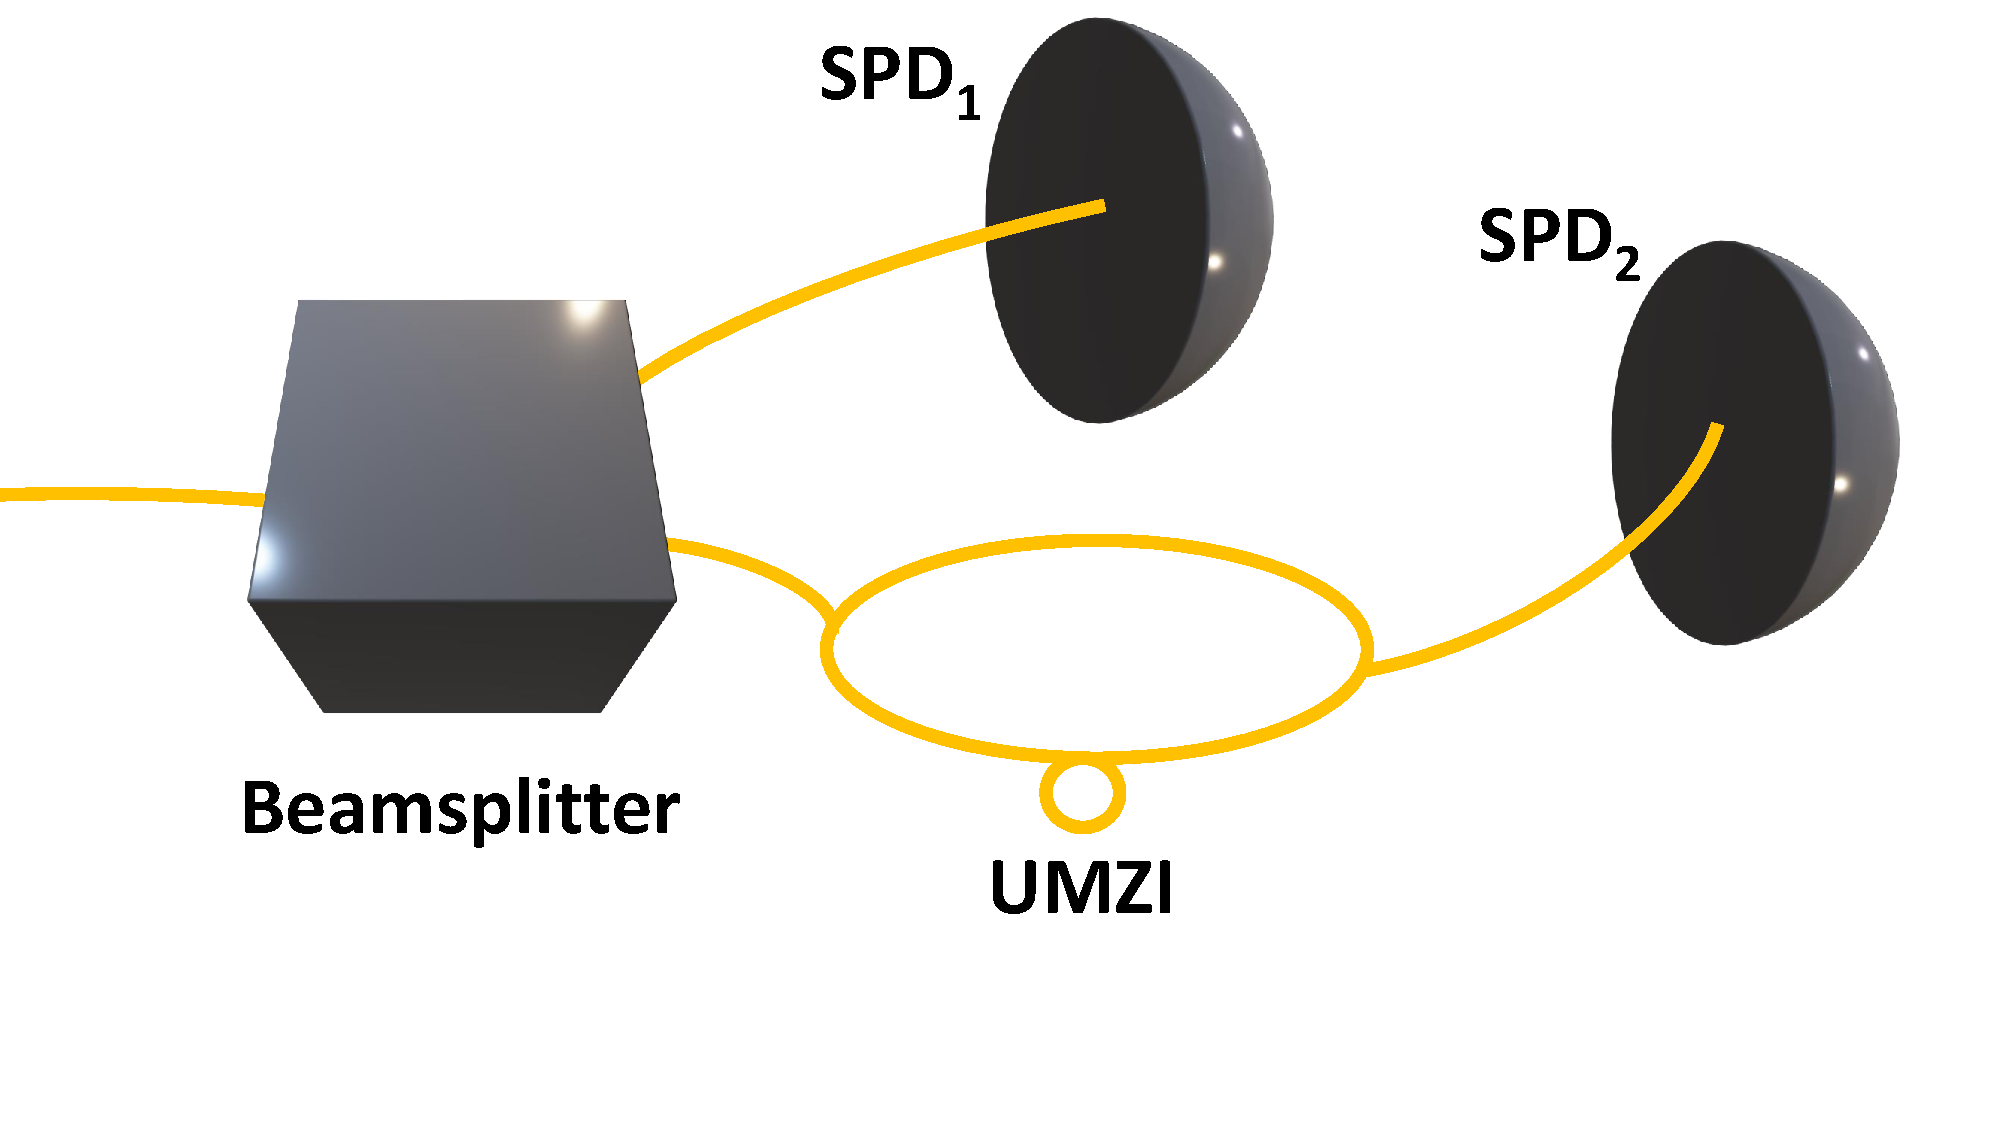
\includegraphics[width=0.6\textwidth, height=6cm]{./figures/Bob.pdf}
        	\label{bob}
    \end{figure}
In the other line half of each pulse interacts with the half of the previous pulse (delayed by 0.5 $T_{bit}$).
\end{description}  


%--------------------------------------------------------------------------------------------------
%------------ SLIDE -------------------------------------------------------------------------------

\mysection{COW - Protocol}\large
The $D_{M2}$ (constructive photon counter) should only click when:
\begin{itemize}
\item A logical bit 1 followed by a logical bit 0 where the coherence is across the bit separation (s=1:0);
\item Decoy state where the coherence is within the bit sequence (s=d);
\end{itemize}
All the other photons should click the $D_{M1}$.
  \begin{figure}[hbt]
    	\centering
    	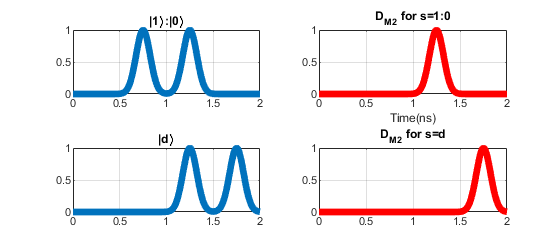
\includegraphics{./figures/Simple2.png}
        	\label{Simple2}
    \end{figure}
%--------------------------------------------------------------------------------------------------
%------------ SLIDE -------------------------------------------------------------------------------

\mysection{COW - Protocol}\large
\vspace*{1cm}
\begin{description}


\item [Step 3] Alice tell Bob the times of the decoy sequences ($2k_d \& 2k_d-1$). Bob also checks if the $D_{M2}$ has ever fired during a $2k_d$ time. Thus they estimate the break of coherence of decoy pulses.

\item [Step 4] Bob reveals the times that he had a detection in $D_{M2}$, Alice verifies if they belong to a $|1\rangle:|0\rangle$, thus, Alice and Bob estimate the break of coherence across the bit separation.

\item [Step 5] Finally, Bob reveals the items that he has detected in the data line. Alice and Bob run error correction and privacy amplification on these bits and end up with a secret key.

\end{description}


%-------------------------------------------------------------------
%------------ SLIDE ------------------------------------------------
\mysection{} \sffamily
\vspace{-10mm}
\large\centerline{E-mail: joaoantonio@ua.pt}
\vspace*{2cm}
\begin{itemize}
	\item Gisin, Nicolas, et al. "Towards practical and fast quantum cryptography." arXiv preprint quant-ph/0411022 (2004).
	\item Branciard, Cyril, et al. "Zero-error attacks and detection statistics in the coherent one-way protocol for quantum cryptography." arXiv preprint quant-ph/0609090 (2006).
	\item Kronberg, Dmitry Anatol'evich, et al. "Analysis of coherent quantum cryptography protocol vulnerability to an active beam-splitting attack." Quantum Electronics 47.2 (2017): 163.
	\item Roberts, George L., et al. "Modulator‐Free Coherent‐One‐Way Quantum Key Distribution." Laser \& Photonics Reviews 11.4 (2017): 1700067.
\end{itemize}

\end{document}